\documentclass[10pt,aspectratio=169,table]{beamer}

\usepackage[utf8]{inputenc}
\usepackage[T1]{fontenc}
\usepackage[spanish]{babel}
\usepackage{graphicx}
\usepackage{booktabs}
\usepackage{array}
\usepackage{enumitem}
\usepackage{hyperref}

\usetheme{Madrid}
\usecolortheme{seahorse}
\setbeamertemplate{navigation symbols}{}
\setbeamerfont{frametitle}{size=\large,series=\bfseries}
\setbeamerfont{footline}{size=\tiny}

\setlist[itemize]{itemsep=2pt,topsep=2pt,parsep=0pt}
\setlist[enumerate]{itemsep=2pt,topsep=2pt,parsep=0pt}

\title[Tarea 1 | Grupo 23]{Tarea 1 | Introducción a la Ciencia de Datos}
\subtitle{Análisis exploratorio del corpus All the News 2.1}
\author[Spoturno \and Buero]{Tomás Alejo Spoturno \and Nicolás Buero}
\institute[FIng, UdelaR]{Facultad de Ingeniería, Universidad de la República}
\date{Mayo 2026, Grupo 23}

\begin{document}

% ========== TAPA ==========
\begin{frame}
  \titlepage
  \begin{center}
    \scriptsize Repo: \url{https://github.com/Nicolasvb23/intro-cd}
  \end{center}
\end{frame}

% ========== SLIDE 2: DATOS Y LIMPIEZA ==========
\begin{frame}{Datos y limpieza}
  \begin{columns}[T]
    \begin{column}{0.48\textwidth}
      \textbf{Dataset}
      \begin{itemize}
        \item 30.213 artículos, 26 medios.
        \item Top 5 (62\%): Reuters, NYT, CNBC, The Hill, People.
      \end{itemize}
      \vspace{0.4em}
      \textbf{Calidad}
      \begin{itemize}
        \item \texttt{author} 38\%, \texttt{section} 34\%, \texttt{article} 4\% nulos.
        \item \texttt{date}: dos formatos $\to$ \texttt{format=mixed}.
        \item \texttt{year/month/day} redundantes con \texttt{date}.
        \item \texttt{month} como \texttt{str} con valores tipo \texttt{"1.0"}.
      \end{itemize}
    \end{column}
    \begin{column}{0.52\textwidth}
      \begin{block}{\texttt{clean\_text}}
        \begin{enumerate}
          \item Minúsculas.
          \item Eliminar URLs.
          \item Puntuación $\to$ espacio (no borrado).
          \item Eliminar números aislados.
          \item Colapsar espacios.
        \end{enumerate}
        \vspace{0.2em}
        \scriptsize\textbf{Campo elegido:} cuerpo del artículo.
      \end{block}
    \end{column}
  \end{columns}
\end{frame}

% ========== SLIDE 3: DISTRIBUCIÓN POR MEDIO ==========
\begin{frame}{Artículos por medio}
  \begin{center}
  \begin{tabular}{lrr}
    \toprule
    \textbf{Medio} & \textbf{Artículos} & \textbf{\% del corpus} \\
    \midrule
    Reuters            & 9.431 & 31,2\% \\
    The New York Times & 2.840 &  9,4\% \\
    CNBC               & 2.623 &  8,7\% \\
    The Hill           & 2.349 &  7,8\% \\
    People             & 1.528 &  5,1\% \\
    \midrule
    \textbf{Top 5}     & \multicolumn{2}{c}{\textbf{62\% del corpus total}} \\
    Otros 21 medios    & 11.442 & 37,9\% \\
    \bottomrule
  \end{tabular}
  \end{center}
  \vspace{0.4em}
  \small Reuters concentra más de la mitad del top-5: su volumen refleja la producción de una \textbf{agencia de cable}, no de una redacción editorial clásica.
\end{frame}

% ========== SLIDE 4a: ARTÍCULOS POR MES ==========
\begin{frame}{Artículos publicados a lo largo del tiempo}
  \centering
  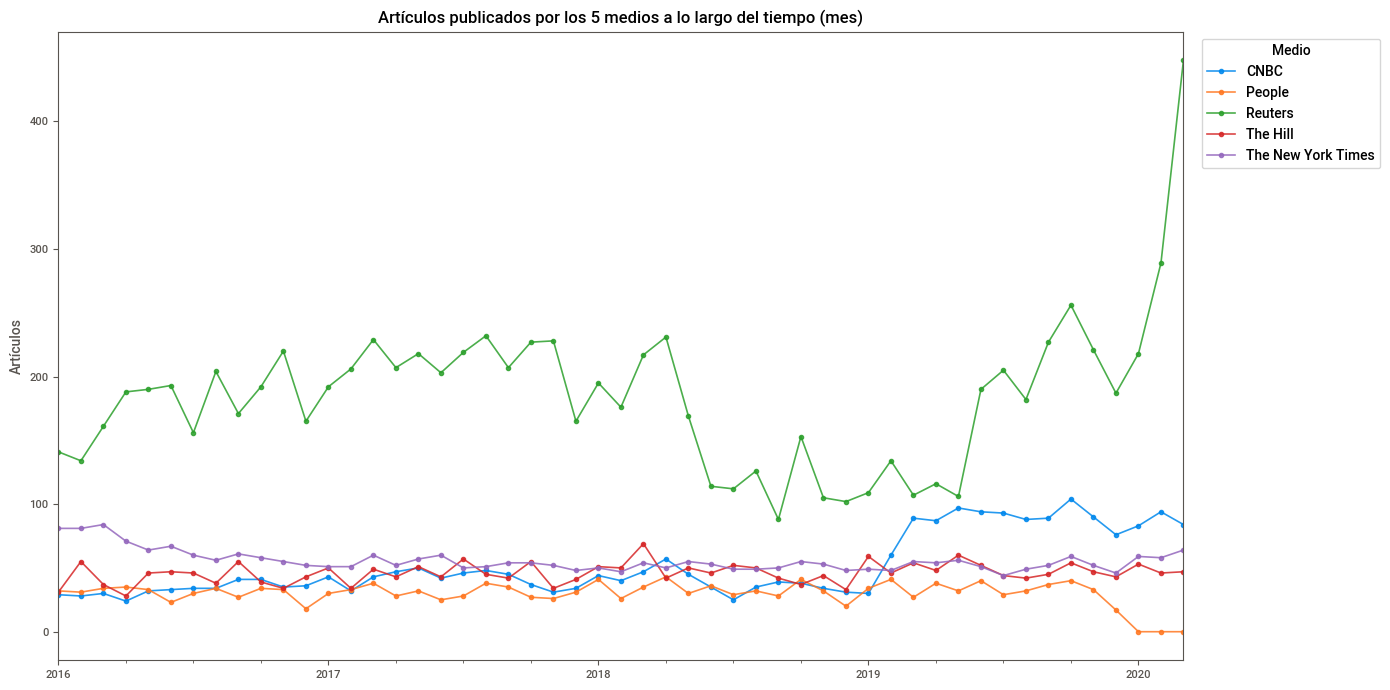
\includegraphics[width=0.92\textwidth,height=0.82\textheight,keepaspectratio]{figs/only_plot.png}
\end{frame}

% ========== SLIDE 4b: ARTÍCULOS POR AÑO ==========
\begin{frame}{Artículos publicados por año}
  \centering
  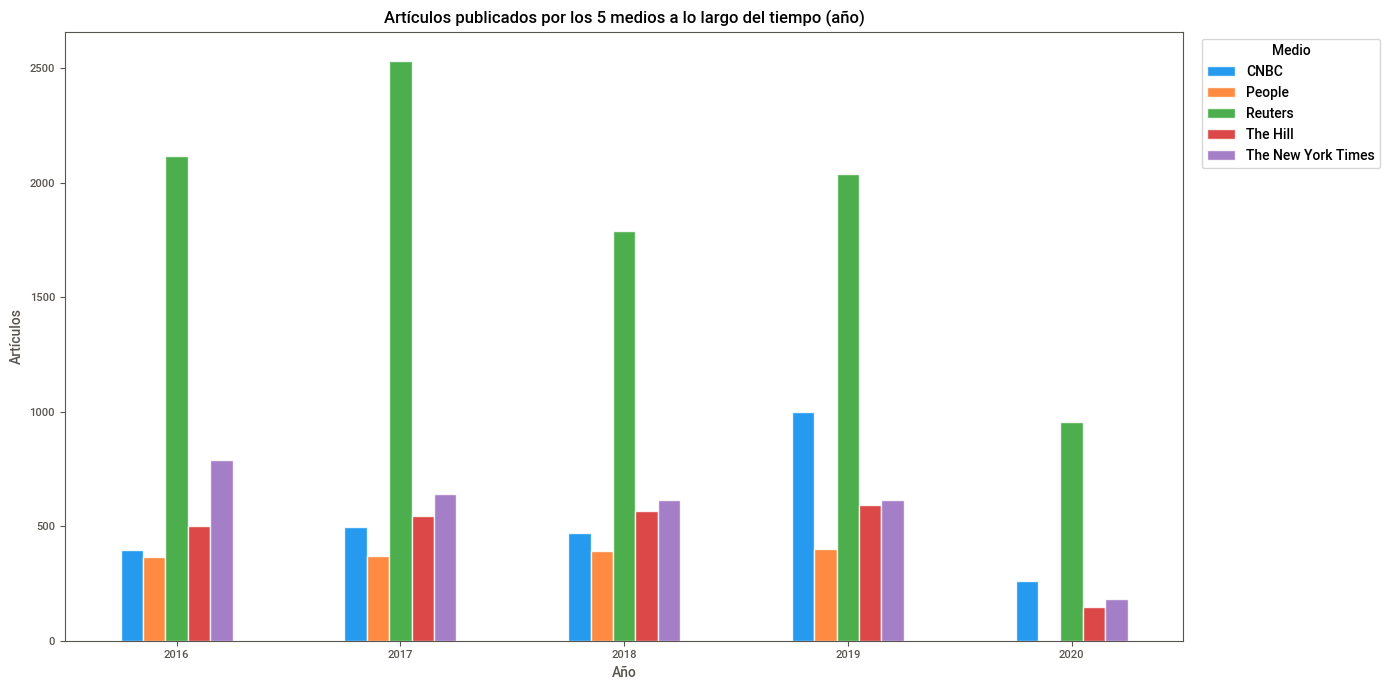
\includegraphics[width=0.92\textwidth,height=0.82\textheight,keepaspectratio]{figs/only_bars.png}
\end{frame}

% ========== SLIDE 5: PATRONES CÍCLICOS ==========
\begin{frame}{Patrones cíclicos de publicación}
  \centering
  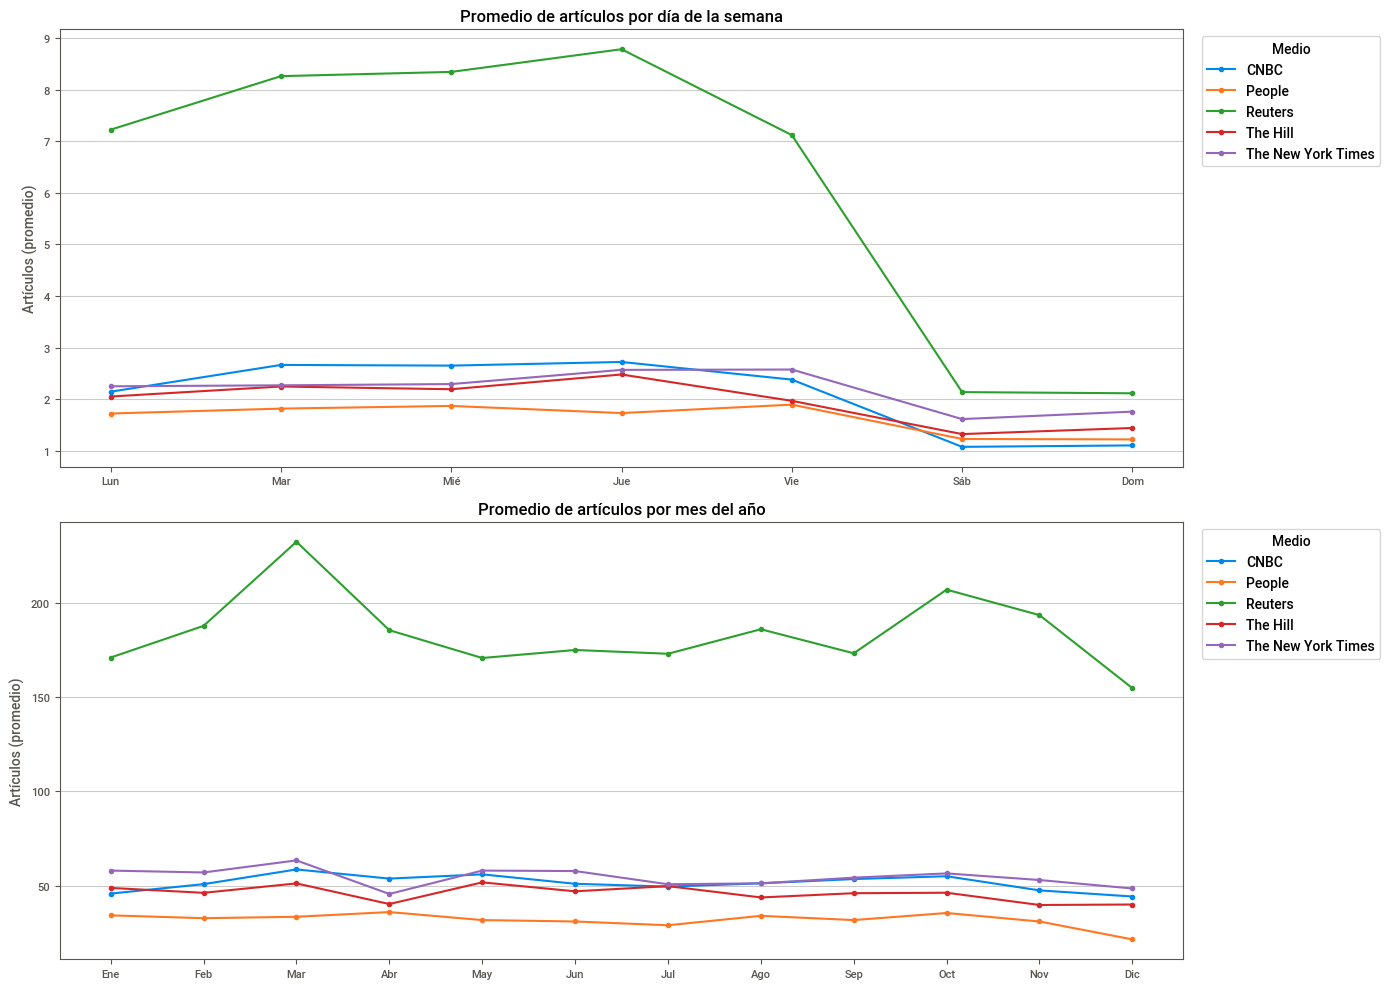
\includegraphics[width=0.88\textwidth,height=0.76\textheight,keepaspectratio]{figs/temporal_dow_month.png}\\
  \vspace{0.3em}
  \scriptsize No se acotó por período: cobertura uniforme 2016-2020, sin argumento fuerte para restringir.
\end{frame}

% ========== SLIDE 6: PISTAS QUE IDENTIFICAN AL MEDIO ==========
\begin{frame}{Pistas que identifican al medio}
  \footnotesize
  \begin{center}
  \begin{tabular}{lccccc}
    \toprule
    \textbf{Patrón} & \textbf{Reuters} & \textbf{NYT} & \textbf{CNBC} & \textbf{The Hill} & \textbf{People} \\
    \midrule
    Reuters dateline \texttt{(Reuters)} & \cellcolor{red!25}\textbf{91{,}9\%} & 0{,}2\% & \cellcolor{orange!25}24{,}3\% & 0{,}1\% & 0{,}0\% \\
    Título \texttt{| TheHill}           & 0{,}0\% & 0{,}0\% & 0{,}0\% & \cellcolor{red!25}\textbf{100\%}   & 0{,}0\% \\
    Footer Capitol Hill                 & 0{,}0\% & 0{,}0\% & 0{,}0\% & \cellcolor{red!25}\textbf{99{,}4\%} & 0{,}0\% \\
    CNBC mencionado en cuerpo           & 0{,}3\% & 0{,}5\% & \cellcolor{red!25}\textbf{34{,}8\%} & 0{,}6\% & 0{,}2\% \\
    \texttt{nytimes.com} en cuerpo      & 0{,}0\% & \cellcolor{red!25}\textbf{8{,}4\%}  & 0{,}0\% & 0{,}0\% & 0{,}0\% \\
    People \texttt{tells/told PEOPLE}   & 0{,}0\% & 0{,}0\% & 0{,}0\% & 0{,}0\% & \cellcolor{red!25}\textbf{28{,}4\%} \\
    \bottomrule
  \end{tabular}
  \end{center}
  \vspace{0.3em}
  \begin{itemize}\small
    \item Cada patrón es casi exclusivo de \textbf{su medio de origen}.
    \item Excepción: dateline y firma de Reuters en CNBC $\to$ CNBC republica cables.
    \item No se acotó por sección: People solo cubre entretenimiento; The Hill no tiene datos de sección.
  \end{itemize}
\end{frame}

% ========== SLIDE 7: PALABRAS FRECUENTES ==========
\begin{frame}{Palabras frecuentes por medio}
  \begin{columns}[T]
    \begin{column}{0.60\textwidth}
      \centering
      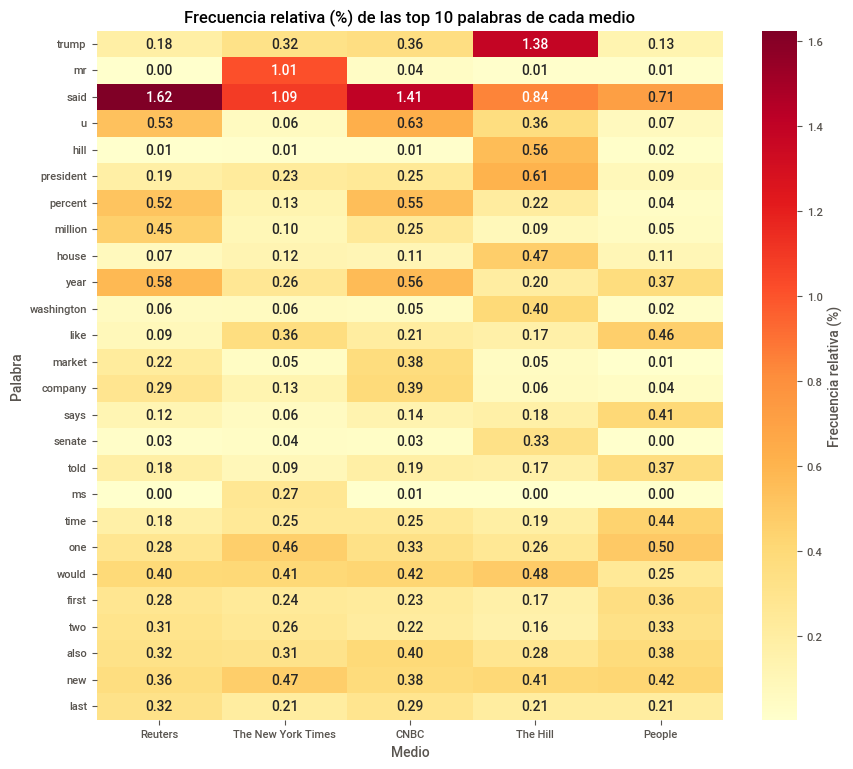
\includegraphics[width=\linewidth,height=0.72\textheight,keepaspectratio]{figs/heatmap_palabras.png}
    \end{column}
    \begin{column}{0.40\textwidth}
      \textbf{Perfiles editoriales claros:}
      \begin{itemize}\small
        \item \textbf{Reuters}: financiero\\
              \textit{percent, company, market}
        \item \textbf{The Hill}: político\\
              \textit{trump, house, senate}
        \item \textbf{People}: celebrities\\
              \textit{family, love, star}
        \item \textbf{NYT \& CNBC}: político-económico
      \end{itemize}
      \vspace{0.5em}
      \small Sin filtrar stopwords los rankings son \textbf{idénticos} entre medios.
    \end{column}
  \end{columns}
\end{frame}

% ========== SLIDE 8: LARGO Y RIQUEZA LÉXICA ==========
\begin{frame}{Largo y riqueza léxica por medio}
  \centering
  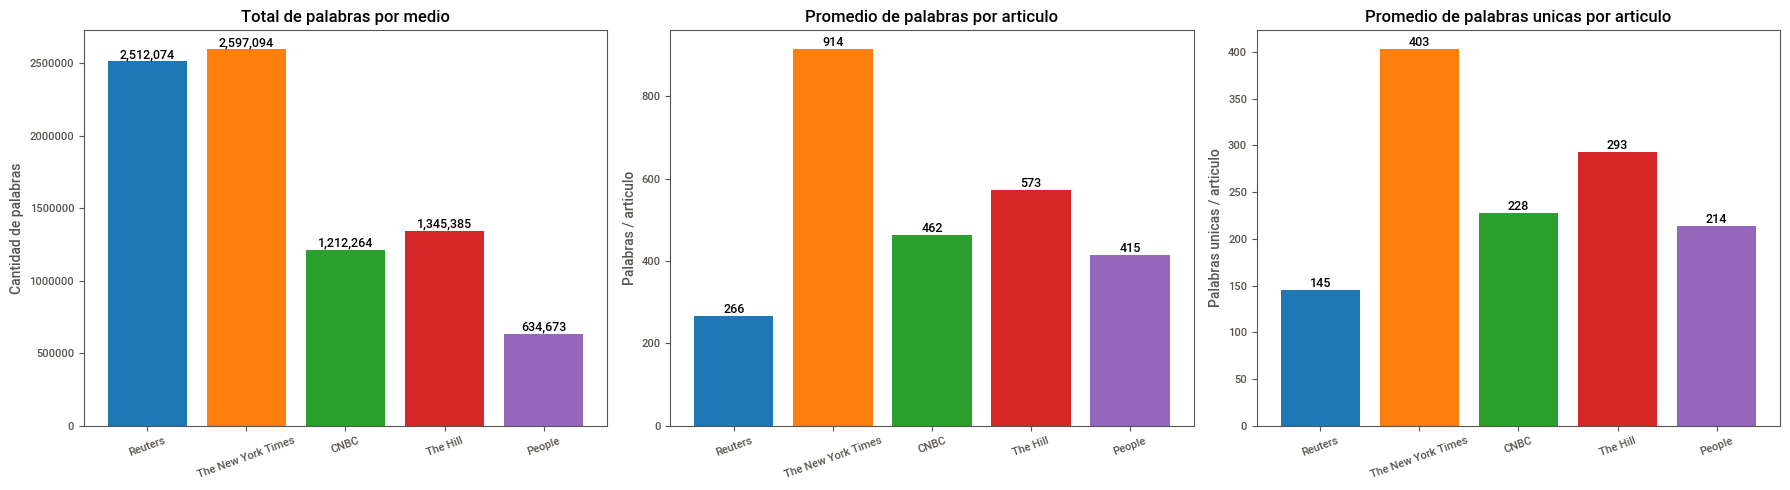
\includegraphics[width=0.95\textwidth,height=0.82\textheight,keepaspectratio]{figs/palabras_por_articulo.png}
\end{frame}

% ========== SLIDE 9: MATRIZ DE MENCIONES ==========
\begin{frame}{Matriz de menciones entre medios}
  \centering
  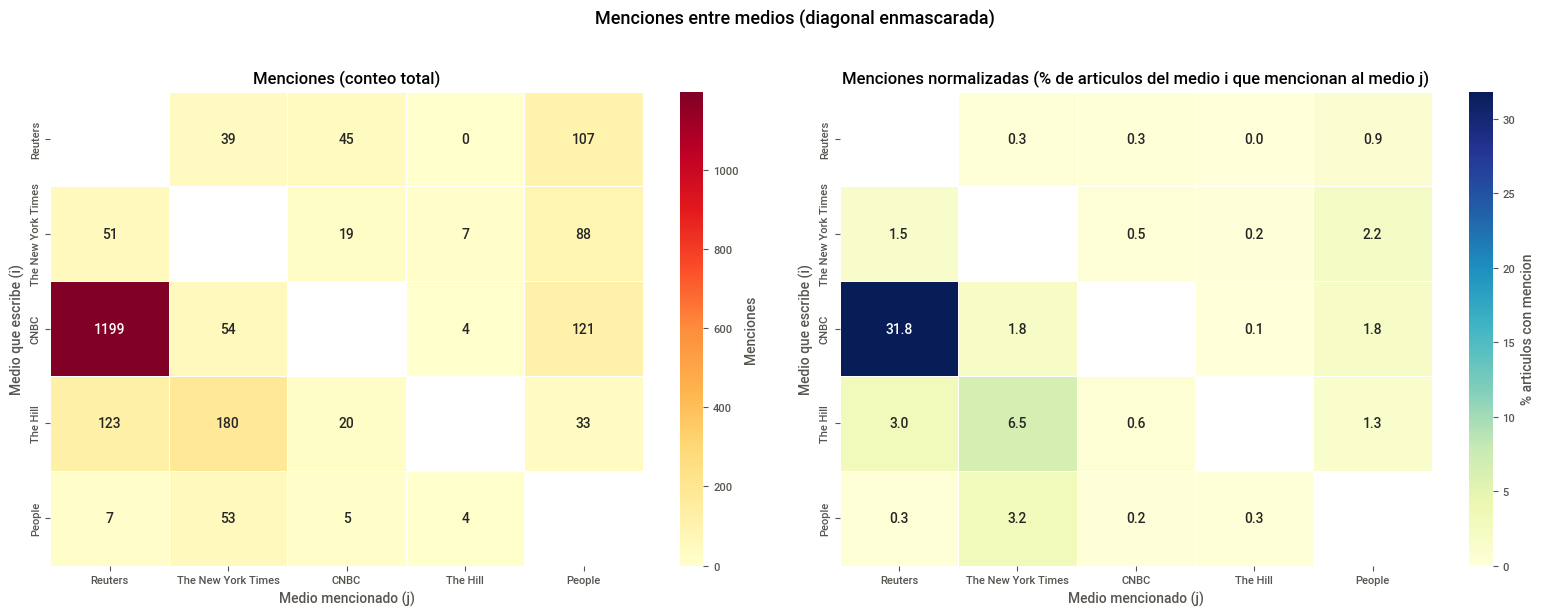
\includegraphics[width=0.92\textwidth,height=0.58\textheight,keepaspectratio]{figs/menciones.png}\\
  \vspace{0.15em}
  \scriptsize Izq: conteo total; der: \% de artículos del medio $i$ que mencionan a $j$. Diagonal enmascarada.\\[0.3em]
  \scriptsize
  \begin{itemize}
    \item \textbf{CNBC} cita Reuters en el \textbf{31{,}8\%} de sus artículos $\to$ republica cables.
    \item \textbf{Asimetría}: The Hill $\to$ NYT (6{,}5\%) pero NYT $\to$ The Hill (0{,}2\%).
    \item \textbf{NYT y People} son autónomos: citan poco a otros (<\,3\%).
    \item \textbf{Truco:} \textit{lookbehind} para detectar \textit{People} (revista) vs.\ \textit{people} (palabra común): solo cuenta precedido de contexto (\texttt{told People}, \texttt{, People reported}).
  \end{itemize}
\end{frame}

% ========== SLIDE 10: CIERRE ==========
\begin{frame}{Preguntas propuestas}
  \textbf{Tres preguntas que abre el análisis:}
  \begin{enumerate}\small
    \item \textbf{Reciprocidad de menciones:} \textquestiondown{}qué pares son simétricos y cuáles asimétricos?
    \item \textbf{Vocabulario distintivo:} \textquestiondown{}qué palabras son propias de un medio, no solo frecuentes?
    \item \textbf{Varianza en el largo:} \textquestiondown{}qué medios son homogéneos y cuáles tienen alta dispersión?
  \end{enumerate}
\end{frame}

% ========== SLIDE 11: GRACIAS ==========
\begin{frame}
  \vfill
  \centering \Huge \textbf{\textexclamdown{}Gracias!}
  \vfill
\end{frame}

\end{document}
